\documentclass[a4paper,12pt]{scrartcl}

\newcommand{\dropsign}[1]{\smash{\llap{\raisebox{-.5\normalbaselineskip}{$#1$\hspace{2\arraycolsep}}}}}%

\usepackage[utf8]{inputenc}
\usepackage[ngerman]{babel}
\usepackage{multicol}
\usepackage{scrpage2}\pagestyle{scrheadings}
\usepackage{graphicx} 
\usepackage{pgfplots}
\usepackage{tikz-timing}

\ihead{Blatt 4, G2B}
\chead{Elena Noll, Sven-Hendrik Haase, E. Böhmecke}
\ohead{\today}
\pagestyle{scrheadings}
\setheadsepline{1pt}
\setcounter{secnumdepth}{0}

\begin{document}

\section{Aufgabe 14}
\subsection{a)}

\definecolor{bgblue}{rgb}{0.41961,0.80784,0.80784}%
\definecolor{bgred}{rgb}{1,0.61569,0.61569}%
\definecolor{fgblue}{rgb}{0,0,0.6}%
\definecolor{fgred}{rgb}{0.6,0,0}%

Encoding von 01100111 \\
\begin{tikztimingtable}[scale=4, timing/slope=0.1]
  01100111            & LHHLLHHH \\
  NRZ-Mark (bipolar)  & LHLLLHLH \\
  Manchester-Code     & lhhlhllhlhhlhlhl \\
  AMI                 & ZHLZZHLH  \\
\extracode
 \makeatletter
 \begin{pgfonlayer}{background}
  % Add background grid lines
  \begin{scope}[gray,semitransparent,semithick]
    %\fulltablegrid{}
    \horlines{}
    \vertlines{}
  \end{scope}
 \end{pgfonlayer}
\end{tikztimingtable}

\subsection{b)}
Wir können in 2 Clocks 1 Bit enkodieren. D.h. wir brauchen allgemein doppelt
so viel Bandbreite wie bei NRZ. Das Besondere beim Manchester-Code ist,
dass das Clock-Signal aus den übermittelten Informationen wieder herauscodiert
werden kann. Dies verhält sich anders bei NRZ.\\
Es ist nicht möglich, dass Datenrate und Schrittgeschwindigkeit gleichgesetzt
werden können, da Schrittgeschwidkeit in Baud gemessen wird und die Datenrate
in Bit pro Sekunde. Die Schrittgeschdigkeit ist ein Teil der ermittelten
Datenrate.

\subsection{c)}
Unter Bitsynchronistation versteht man das "rechtzeitige" auslesen des Signals
zu regelmäßigen, diskreten Zeitabschnitten. Ja, der Manchester-Code
unterstützt Bitsynchronistation, da es selbsttaktend ist und seine
Taktinformation im übertragenen Signal nicht verloren geht. Wenn dies nicht
durch die Codierung selbst gewährleistet werden kann,
muss von außen aufgepasst werden, damit kein "Bit Slipping" erfolgt.

\section{Aufgabe 15}
\subsection{a)}
434790 KHz - 433050 KHz = 1740 KHz (Durchlassbereich)
1740 KHz / 16 KHz = 108,75. D.h. 108 bidirektionale Sprachkanäle passen
in diesen Durchlassbereich.

\section{Aufgabe 16}
\subsection{a)}
Das "Bit stuffing" wird im HDLC-Protokoll eingesetzt um zu vermeiden das innerhab des Datenbereichs bz der Prüfsumme das Opening bzw Closing flag (Bitfolge: 01111110) auftritt.
\begin{itemize}
	\item Bitfolge: 0011111110001111101
	\item Bitfolge nach dem "Bit stuffing": 001111101100011111001
\end{itemize}
\subsection{b)}
Das Bitmuster 01111110 ist als Synchronisationszeichen geeignet, alleridngs nur solange "Bit stuffing" nach 5 aufeinanderfolgenden Einsene ingesetzt wird. Sonst könnte es vorkommen dass in den Nutzdaten zufällig die selbe Bitfolge haben wie das Synchronisationszeichen.
\subsection{c)}
Man kann mit Opening bzw. Closing Frames arbeiten. Somit weiß man wann ein Datenblock anfängt und wo er aufhört. Beim nächsten Opening Frame kann dann der jeweilige Block wieder Synchronisiert werden.
\subsection{d)}
\subsection{Ethernet}
Blocksynchronisation durch MAC-Frames (Media Access Control). Diese bestehen jeweils aus einer Präambel (7 Byte lange alternierende Bitfolge "101010...1010") gefolgt von einem Start Frame Delimeter (SFD). Die alternierende Bitfolge ermöglicht die Bitsynchronisation und das SFD (Blockanfang) die Blocksynchronisation.
\subsection{IEEE 802.11g WLANs}

\section{Aufgabe 17}
\subsection{a)}
\begin{itemize}
	\item Studen: ld(n)
	\item Knoten pro Stufe: n/2
\end{itemize}
\subsection{b)}
\begin{center}
  \makebox[\textwidth]{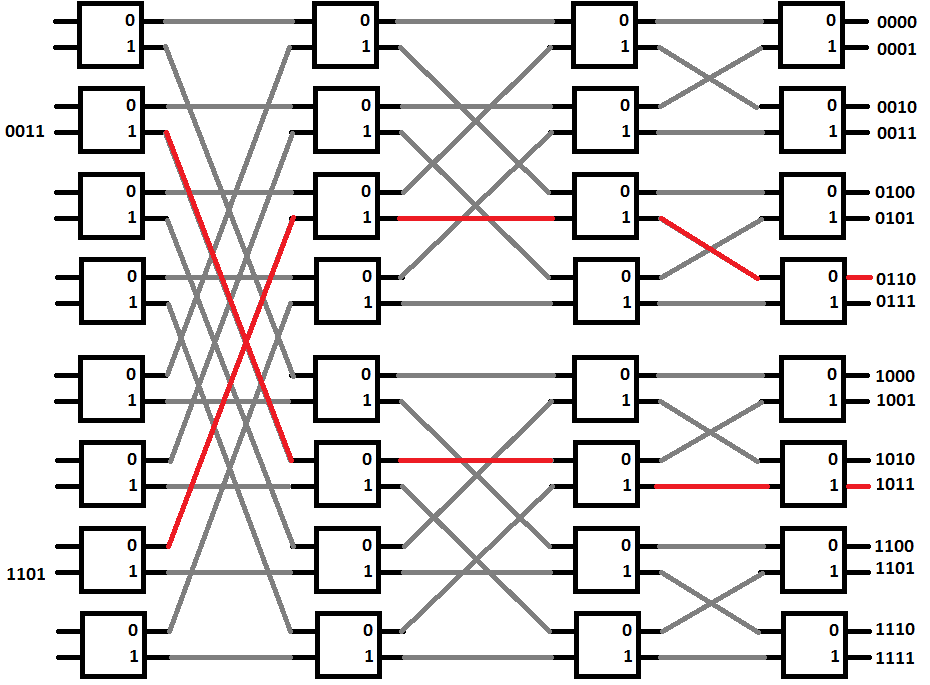
\includegraphics[width=\paperwidth]{./images/Blatt-4-Aufgabe17b}}
\end{center}
Die Zellen blockieren sich nicht auf dem Weg.
\subsection{c)}
Internet Blockierungen in einen Banyan-Netz lassen sich durch folgende Maßnahmen entschärfen:
\begin{itemize}
	\item Sort/Banyan-Netze: vorsortierung von Packeten sodass interne Blockierung vermieden wird
	\item Warteschlangen: Führt dazu dass die Leitung nur von jeweils eine Anfrage zur Zeit durchlässt.
\end{itemize}
\subsection{d)}
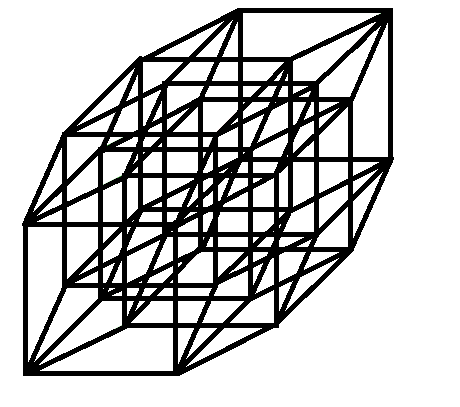
\includegraphics{./images/Blatt-4-Aufgabe17d}\\
Der 5-dimensionale Hperwürfel enthält 32 Knoten, 80 Verbindungen und 5 maximale "Hops" zwischen zwei Knoten. Da jeder Knoten 5 ausgehende Verbindungen jeweils hat, kann ein Ausfall von 5 Verbindung im ungünstigsten Fall bedeuten das 1 Knoten überhaupt nicht mehr durch eine Verbindung erreichtbar ist und somit ist auch nicht mehr sichergestellt das jeder mit jedem Knoten kommunizieren kann.

\subsection{e)}
Diese Topologie kommt bei großen Rechnerclustern zum Einsatz. Es gab auch
Supercomputer, die diese Architektur benutzten, namentlich die Connection
Machine.

\end{document}
